\documentclass[conference]{IEEEtran}
% *** CITATION PACKAGES ***
%
\ifCLASSOPTIONcompsoc
  % IEEE Computer Society needs nocompress option
  % requires cite.sty v4.0 or later (November 2003)
  \usepackage[nocompress]{cite}
\else
  % normal IEEE
  \usepackage{cite}
\fi
\usepackage{amsmath,amssymb,amsfonts}
\usepackage{algorithmic}
\usepackage{graphicx}
\usepackage{textcomp}
\usepackage{xcolor}
\usepackage{caption}
\usepackage{hyperref}
\usepackage{float}
\def\BibTeX{{\rm B\kern-.05em{\sc i\kern-.025em b}\kern-.08em
    T\kern-.1667em\lower.7ex\hbox{E}\kern-.125emX}}

\makeatletter
\newcommand{\linebreakand}{%
  \end{@IEEEauthorhalign}
  \hfill\mbox{}\par
  \mbox{}\hfill\begin{@IEEEauthorhalign}
}
\makeatother
% ==================================
% END
% ==================================


\begin{document}

\title{Contrastive Recognition Through Extraction}

% ------------------------------------ %
\author{
\IEEEauthorblockN{Seth Grief-Albert}

\and
\IEEEauthorblockN{Aidan Kinnear}

\and
\IEEEauthorblockN{Dharsan Ravindran}

\and
\IEEEauthorblockN{Vivek Chokkalingam}

\and
\IEEEauthorblockN{Arya Farivar}

\linebreakand
\IEEEauthorblockA{
    \text{Queen's University}, \textbf{QMIND} \\
    \{seth.griefalbert, 21adk1, 20vdc1, 19dr26, 22sw59\}@queensu.ca
}
} % end authors
% ------------------------------------ %

\maketitle

\begin{abstract}

The world as we perceive it is multimodal: we learn about and interact with our environments through our perceptions. Large Language Models (LLMs) have emerged in artificial intelligence as natural language processing engines that form textual generations based on their inputs. We observe that LLMs form relationships between objects and their environments during pre-training. We propose Contrastive Recognition Through Extraction (CoRTEx), a novel framework that expands the information content of image-captioning models while grounding generations in observed visual features through a discriminator. We leverage the reasoning capabilities of a base model and encourage it to create vivid descriptions through fine-tuning on a descriptive instruction-tuning dataset. We release code on GitHub and model adapter on Hugging Face: \url{https://github.com/SethGA/CoRTEx}, \url{https://huggingface.co/SethGA/neocortex-grounded}.

\end{abstract}

\section{Introduction}

Multimodal LLMs have shown increasing prevalence throughout the field of artificial intelligence. These LLMs can be leveraged for their pre-training knowledge to form linguistic shortcuts that aid in the task of downstream question-and-response on visual content \cite{ko2023large}. These models, however, can often over rely on questions and become ungrounded to observed visual features, leading to linguistic bias. A research area of interest in artificial intelligence is Computer Vision in the Wild, which aims to develop generalizable computer vision that can be deployed in novel contexts \cite{li2022elevater}. Linguistic bias is a key unsolved problem in this area. Recently, BLIP-2 has emerged as a State-of-the-Art image captioning model \cite{li2023blip2}. Particularly compelling is its ability to produce zero-shot captions that are well-grounded in image features, but lack in detail and complexity. Yet, if the hallucination problem is re-framed as an inference problem, then by controlling the level of hallucination, more comprehensive descriptions can be generated. We leverage this existing capability of LLMs to form a cohesive understanding of environments captured in videos.

\textbf{Our Contributions}: We explore the grounding of zero-shot image captioning generations for video understanding, and use a discriminator model to construct a scene memory that can be used for downstream tasks including Visual Question Answering. We expand on the work of LLaMA-VQA \cite{ko2023large} and utilize the latent knowledge of LLMs learned during pre-training, fine-tuning LLaMA-2 to create rich descriptions from image captions. The discriminator computes the similarity between these descriptions and the grounded visual feature memory to supervise the hallucination rate of our model.

\section{Related Works}
\noindent
\textbf{Multimodal Instruction Tuning}:
\\
Although end-to-end fine-tuning of LLMs is computationally expensive, parameter-efficient fine-tuning techniques including Low-Rank Adaptation have demonstrated comparable results through the introduction of a smaller weight matrix concatenated with the language model \cite{xu2023parameterefficient}\cite{hu2021lora}. LLaMA-Adapter proposed a zero-initialized attention mechanism to adapt a relatively small number of learnable parameters to a frozen base model such as LLaMA, which lent itself well to image inputs using a visual encoder like CLIP\cite{zhang2023llamaadapter}\cite{radford2021learning}. During pre-training, LLMs learn the relationships between objects. If language models can be made to "see" through the introduction of visual encoders, existing understanding of these relationships can be effectively leveraged.
\\
\textbf{Visual Question Answering}:
\\
Several recent advances in developing general-purpose assistants have included visual question answering (VQA) as a key focus, including Flamingo and Vicuna \cite{alayrac2022flamingo}\cite{vicuna2023}. By fine-tuning an LLM on the output of a visual encoder, a model can answer natural-language questions about both visual and video context \cite{liu2023visual}. However, many such fine-tuning implementations have utilized multiple choice question-and-answer instruction tuning, which can lead to hallucinations from over-reliance on question content \cite{ko2023large}. Other VQA approaches have used detailed prompting to assist the model in generating descriptions of visual content, like in VideoChat \cite{li2024videochat}. Our approach moves towards zero-shot video descriptions through fine-tuning. We build upon the work of LLaMA-VQA to capitalize on \textit{linguistic shortcuts} for semantic relationship modelling while reducing hallucinations. Our model architecture includes a \textit{discriminator} that compares descriptive generations to a grounded \textit{visual feature memory}.
\\
\textbf{World Model}:
\\
A world model for an LLM is an internal state representation of an observed environment. Language models have been shown to have more rigorous reasoning capabilities in physical contexts when exposed to embodied experience data \cite{xiang2023language}. Reasoning via Planning is a recent framework to adapt world-modelling and enhanced reasoning capabilities to LLMs \cite{hao2023reasoning}. Our work builds upon the knowledge that an LLM has learned during pre-training to construct a small semantic world model we call \textit{world memory}.

\section{Visual Feature Memory}

LLMs are engines of language. Efforts to extend their capabilities to the real world have proved challenging, especially due to their lack of visual perception. A key advantage that LLMs, and transformer architectures in general, have over traditional machine learning approaches is their scalability. It seems worthwhile to explore how textual capabilities can be applied to real-world tasks, but a key problem arises: How can we effectively interface LLMs with the world if they cannot process their environments? To build semantic context from a video environment, we first propose a visual feature memory $F_m$ to ground the language model in real observations. We utilize BLIP-2 inference on each relevant video frame to form our grounding captions. A caption usually consists of a short, 5-10 word description of one image frame. The Python Natural Language Toolkit is used to extract the object features present in each frame, capturing their frequency and storing them in a permanent feature list. This list acts as a query database, which can be indexed and processed to aid in reducing hallucinations downstream.

\section{CoRTEx}

\subsection{Architecture}

We aim to build a semantic world memory $M_W$ through a video input $V$. Each video frame $\langle v_{1}\rangle,\langle v_{2}\rangle,\dots,\langle v_{n}\rangle$ captured at time $t_{1},t_{2}\dots,t_{n}$ is input into BLIP-2 to create a list of captions $\vec c=[c_{1},c_{2},\dots,c_{n}]$. The generator model $G$ and visual feature memory $F_m$ take $\vec c$ to generate a detailed scene description and feature list respectively \ref{gen} \ref{vfm}.

\begin{equation} \label{gen}
G(\vec c)=d
\end{equation}

\begin{equation} \label{vfm}
F_m(\vec c)=[f_{1},f_{2},\dots, f_{k}]
\end{equation}

Where $d$ is the generated description and $f$ is an image feature.

\begin{figure}[H]
\centering
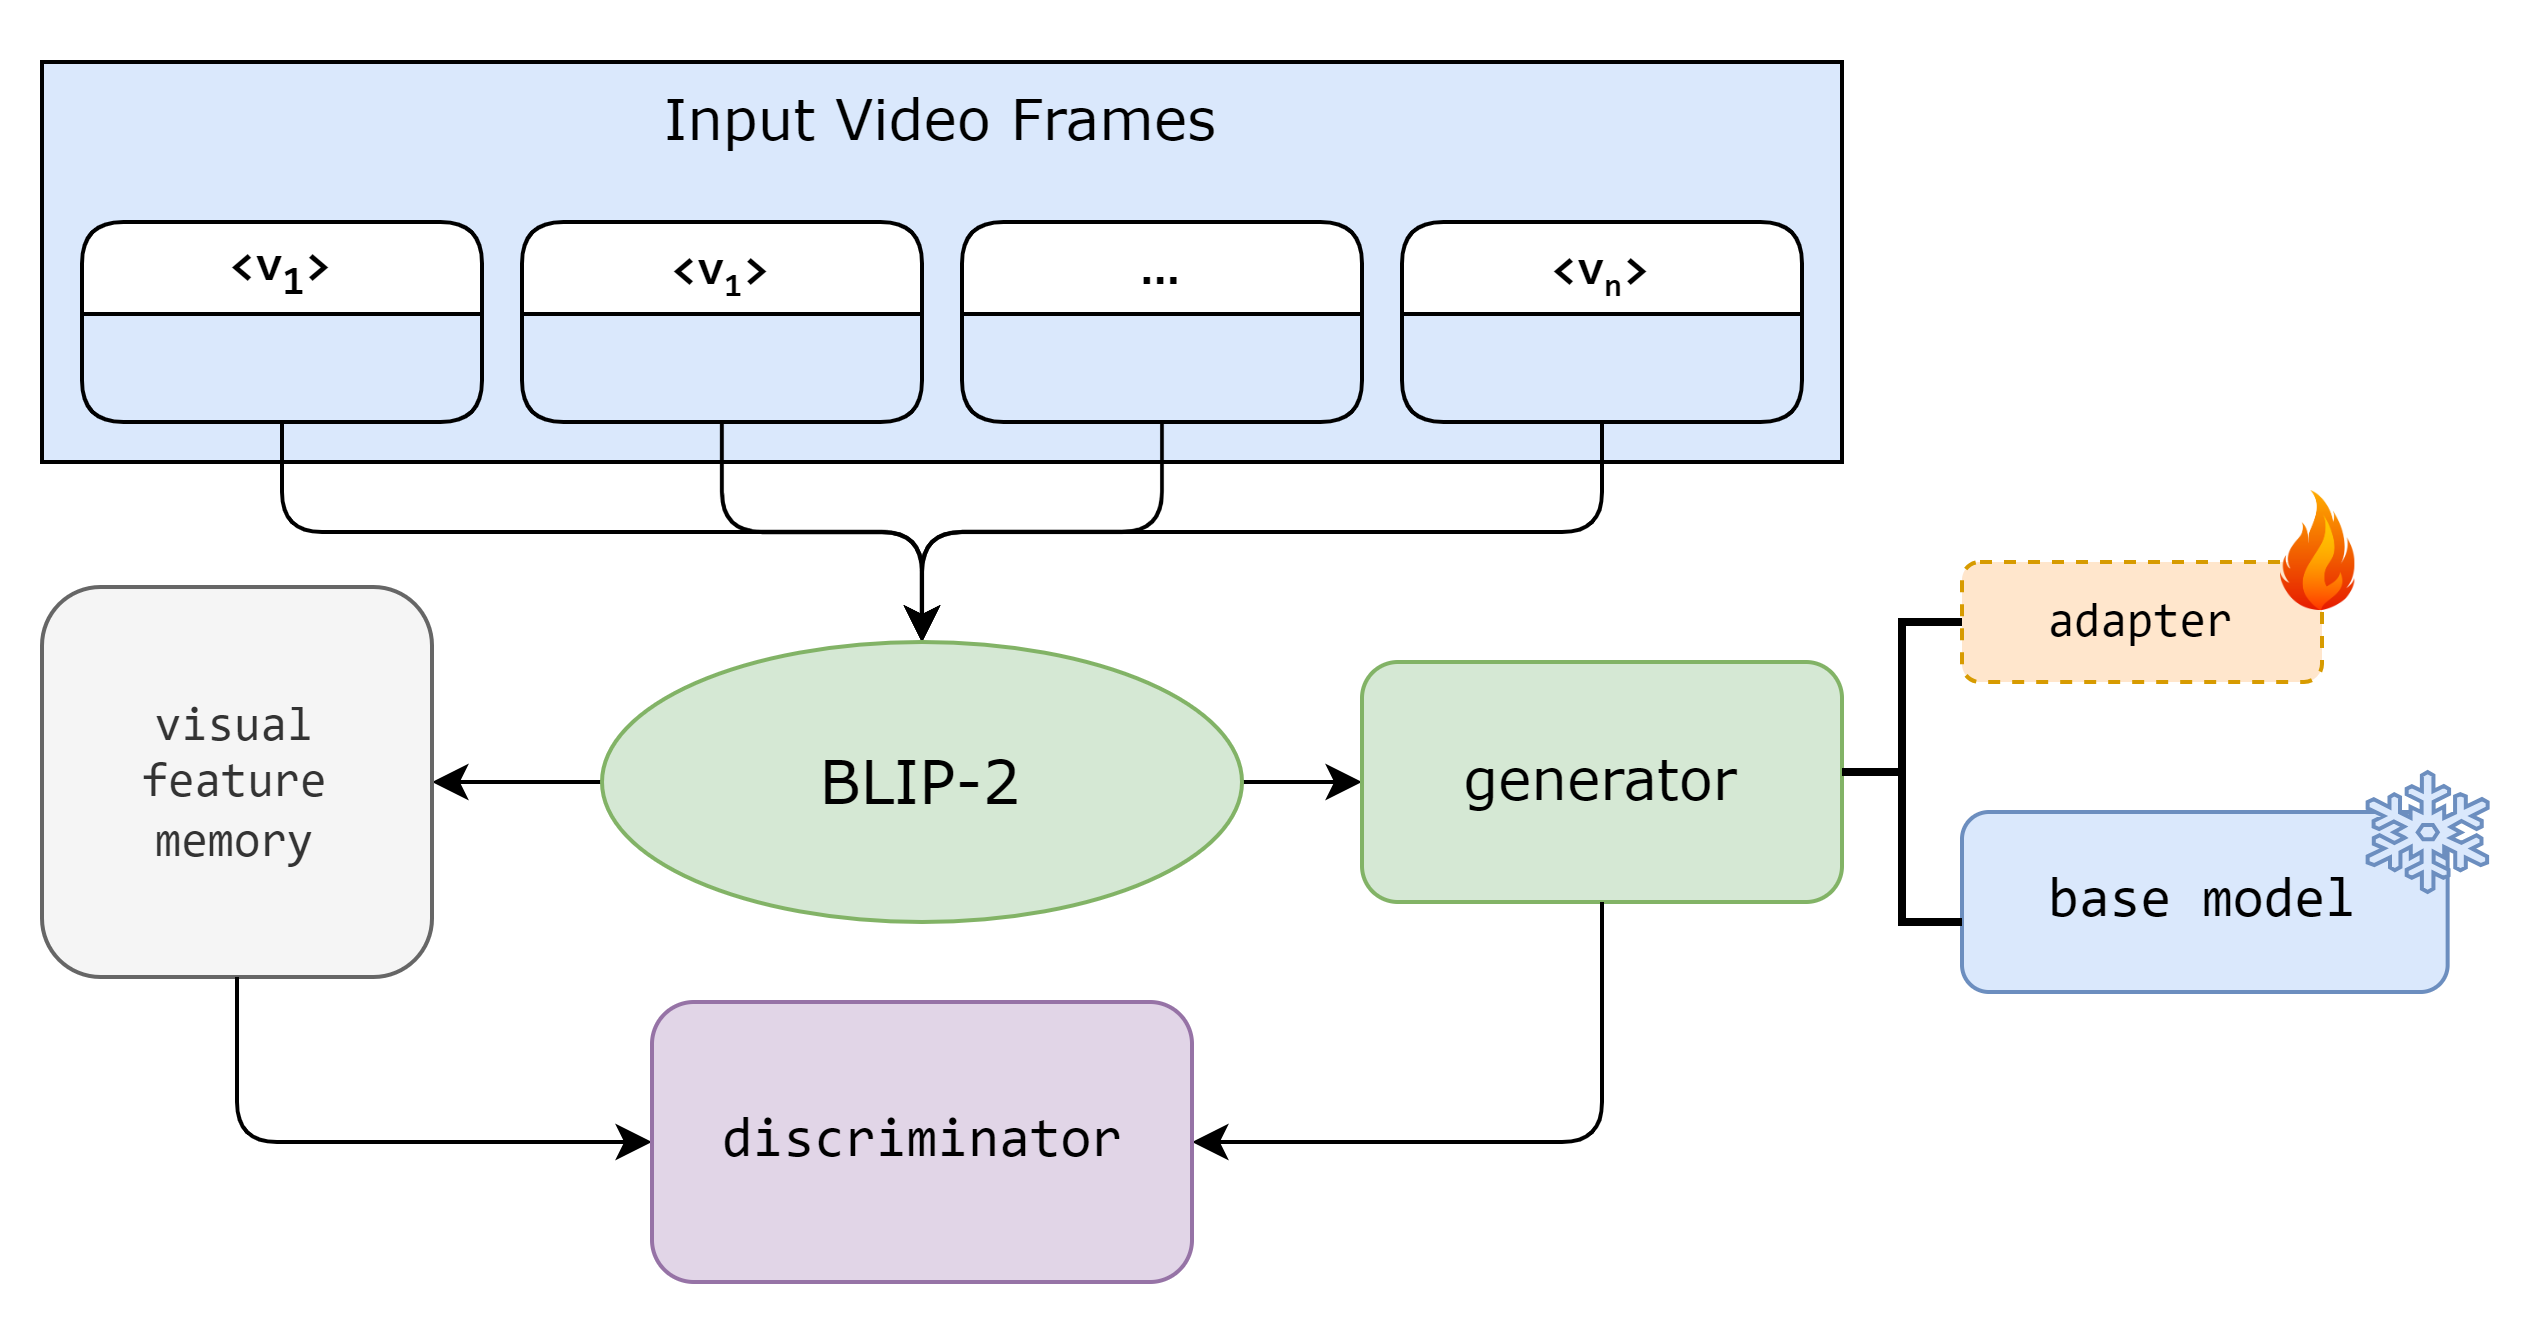
\includegraphics[width=\columnwidth]{cortex.png}
\caption{CoRTEx Architecture Diagram}
\label{fig:image}
\end{figure}

\subsection{Training}

We construct the neocortex\_grounded\_23k dataset in alpaca instruction tuning format from the detailed description dataset proposed in Visual Instruction Tuning \cite{liu2023visual}. Both datasets are based upon the train\_2014 COCO dataset \cite{lin2015microsoft}. In addition to the generations within detail\_23k, we add the human annotations as input to the model, corresponding to a similar BLIP-2 caption.

\begin{table}[h] % You might want to use the table environment for better placement
\centering
\begin{tabular}{ |l|l|l| } 
 \hline
 Video: $\langle v_1\rangle$, $\langle v_2\rangle$, \dots, $\langle v_n\rangle$\\ 
 Descriptive question: $q$\\ 
 Human Annotation: $\langle c_{H_1}\rangle$, $\langle c_{H_2}\rangle$, \dots, $\langle c_{H_5}\rangle$\\
 Synthetic Annotation: $\langle c_S\rangle$ \\
 \hline
\end{tabular}
\caption*{Table 1: neocortex-grounded-23k dataset construction}
\end{table}

We fine-tune our model using 2$\times$A40 GPUs, on LLaMA-2-7b-hf from Meta and NousResearch. We fine-tune on the neocortex\_grounded\_23k dataset for 3 epochs, with a learning rate of 2e-4.

\subsection{Few-shot Scene Discrimination}

The goal of the discriminator is to compare how similar the generated scene description is to the visual feature memory by measuring the hallucination occurrence through cosine similarity.

\begin{figure}[H]
\centering
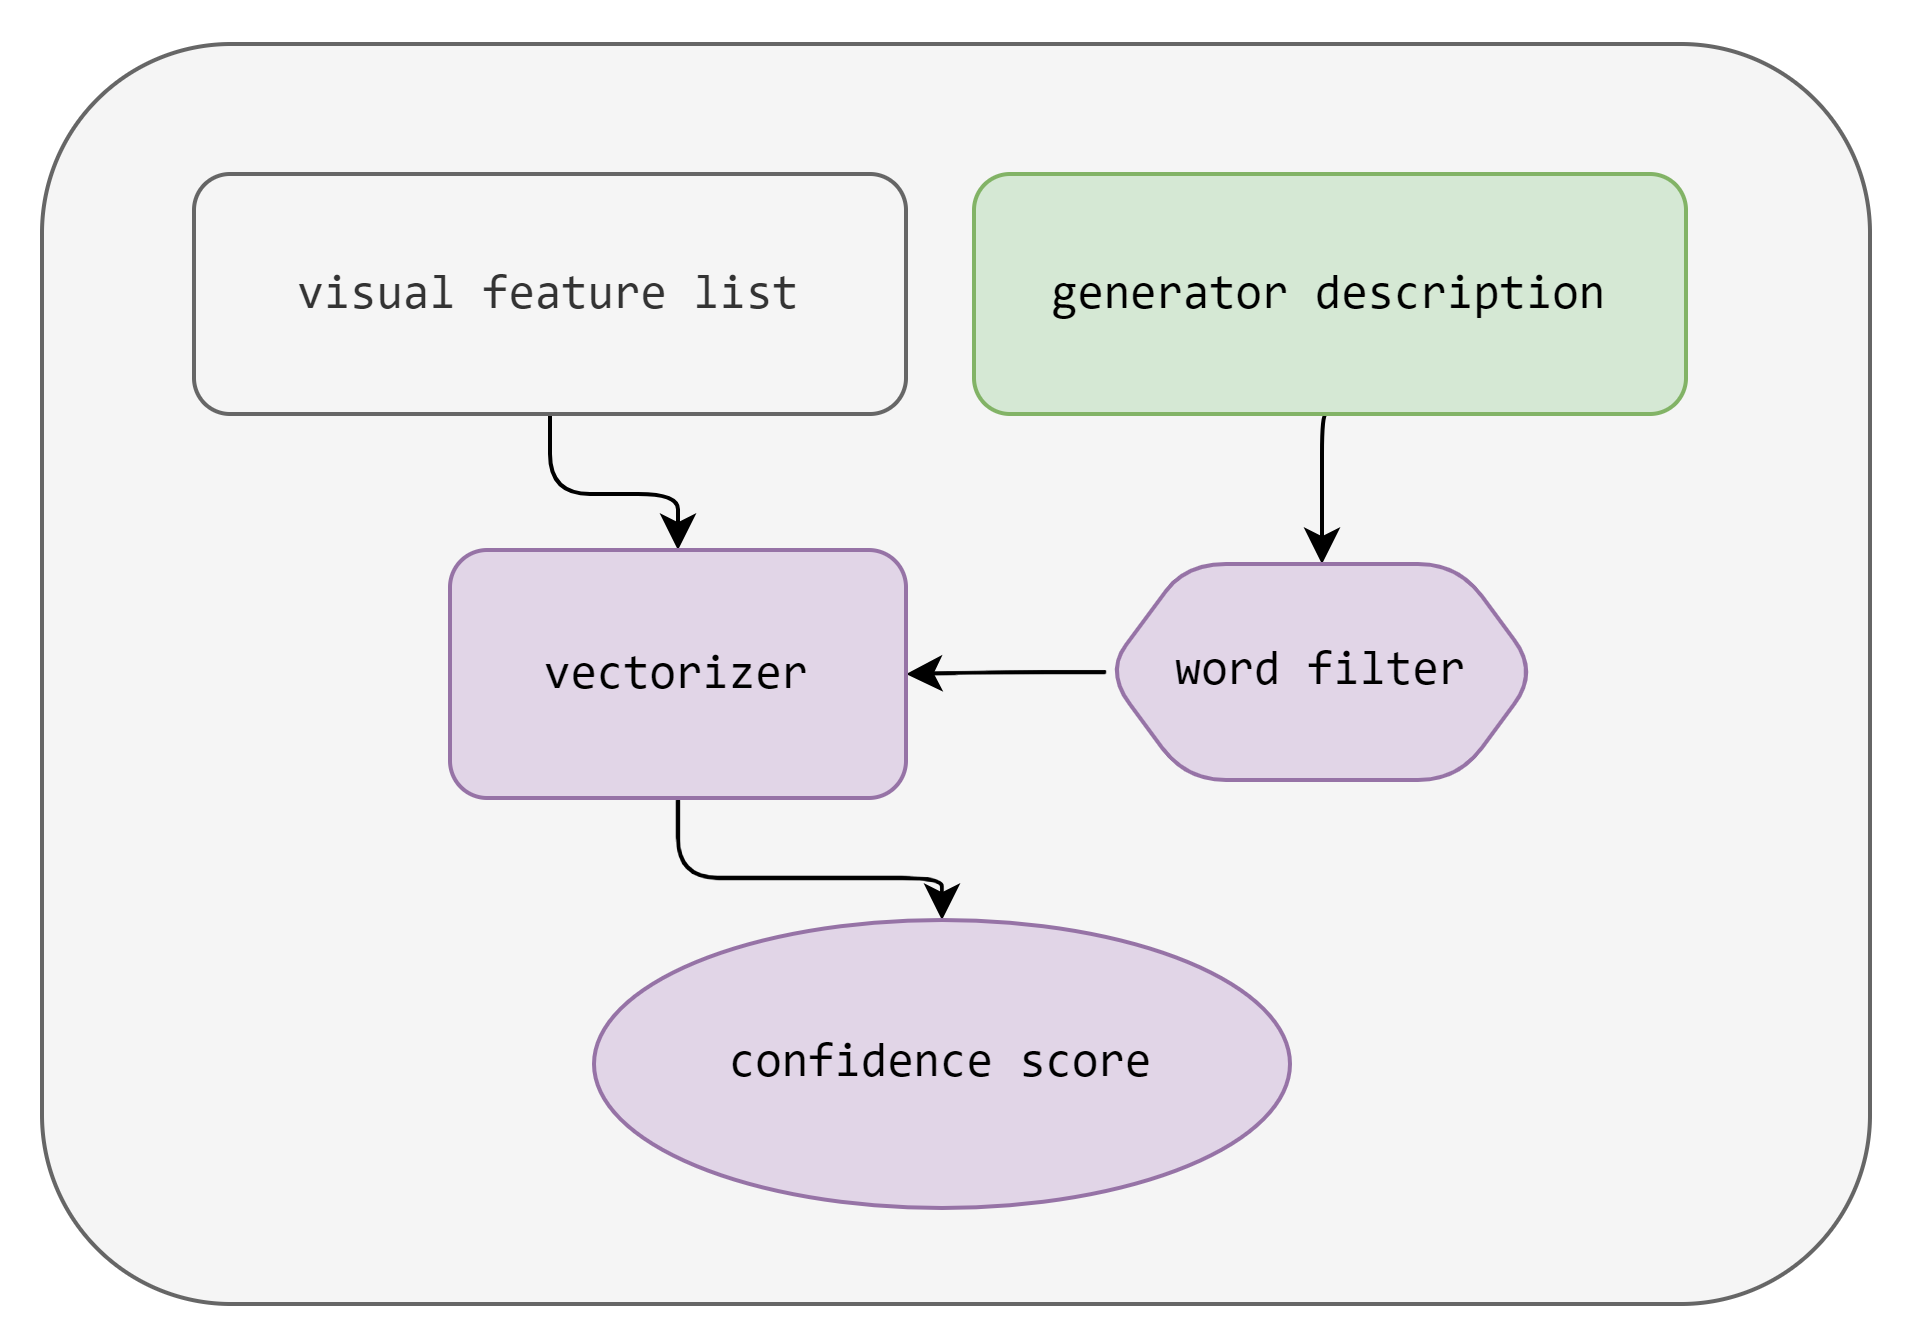
\includegraphics[width=\columnwidth]{discriminator.png}
\caption{CoRTEx Discriminator Diagram}
\label{fig:image}
\end{figure}

The discriminator retrieves a list of features from the visual feature memory, and the corresponding generated description of the input video. First, the generated description is filtered to remove insignificant words and punctuation, resulting in a string of words each separated by a space, to match the format of the feature list. This creates a pool of words, both obtained by the visual feature memory and the generator. We create a vector for both the feature list and the generated description. The vectors contain the frequency of the words used in each string, respectively. The size of the vector is determined by the number of words in the union of the feature list and generated description.

We compare the vectors on word commonality with respect to the corpus, using Term Frequency-Inverse Document Frequency (TF-IDF) to return a float value between 0-1 for each word in the vector \ref{TF-IDF}.

\begin{equation} \label{TF-IDF}
w_{i,j} = tf_{i,j} \cdot \log \left( \frac{N}{d_i} \right)
\end{equation}

Where $tf_{i,j}$ is the frequency of $i$ in $j$ divided by the total number of words in $j$, $N$ is the total number of documents, and $d_i$ is the number of documents containing $i$. A cosine similarity function is used to determine a confidence score that the generated description is grounded in the visual feature memory \ref{cosine}. Cosine similarity is especially useful for computing the similarity of sparse data within text documents.

\begin{equation} \label{cosine}
S_{C}(A,B)=\frac{A\cdot B}{||A||\cdot||B||}=\frac{\sum\limits_{i=1}^{n}A_{i}B_{i}}{\sqrt{\sum\limits_{i=1}^{n}A_{i}^{2}}\cdot\sqrt{\sum\limits_{i=1}^{n}}B_{i}^{2}}
\end{equation}
Where $A$ and $B$ are vectors of the same length. The cosine similarity of the two vectors ($S_C$) is appended to the generated description to form the world memory $M_W=d,S_C$ for use in downstream tasks.

\section{Experiments}

We test our model on multiple video environments with varying scene complexity. The captions generated from BLIP-2 give grounded depictions of each frame, allowing for our fine-tuned model to build upon these captions. Our model builds upon the image captions and the pre-training knowledge of LLaMA-2 to construct a human-like description of the scene. In \ref{fig:beach}, our model uses its existing knowledge of beaches to essentially "dream" about what it is looking at. This description includes the experience of the beach-goers in regards to their sentiment and the weather, which the BLIP-2 captions provide no information on; the generator infers that the presence of many people is an implication that the weather is pleasant. These insights provide a more detailed understanding of the big picture of the scene and shows the capabilities of our model for grounded textual expansion. The corresponding confidence score given by the discriminator shows reasonable similarity from the generated description and feature list. 

\begin{figure}[H] 
\centering
\includegraphics[width=\columnwidth]{EXP_beach.png}
\caption{Beach Scene Experiment}
\label{fig:beach}
\end{figure}

Longer temporal context can be absorbed by our model to improve its world memory over time. In \ref{fig:traffic}, the camera is moved in a panorama around a busy intersection. The model pieces together the various frame captions into a cohesive understanding of the environment being captured.

\begin{figure}[H]
\centering
\includegraphics[width=\columnwidth]{EXP_traffic.png}
\caption{Traffic Scene Experiment}
\label{fig:traffic}
\end{figure}

\subsection{Limitations}

The CoRTEx architecture creates a mental model of a video scene we call world memory. One limitation to this approach is that specific events within the video can be lost, as our generator model produces a description of the entire scene as if it was a static image. In the future, we can explore forming multiple and continuous world memories to be used in downstream visual question answering. The discriminator is implemented to gauge the hallucination rate of the generator. Establishing a threshold for an acceptable hallucination rate such that the model could effectively use its pre-training knowledge could open a path to training the generator and discriminator with a traditional GAN architecture \cite{goodfellow2014generative}. Although reliable data accessibility remains a challenge, novel approaches towards synthetic data creation could prove lucrative. Additionally, we rely on BLIP-2 as a "grounded" image captioning model. Future work could implement CLIP as a visual encoder, in which image features to the word embedding space through a linear layer, as proposed in Visual Instruction Tuning \cite{liu2023visual}.

\section{Conclusion}

We propose CoRTEx, an architecture leveraging LLaMA-2, fine-tuned on synthetic video annotations, and BLIP-2 captions to build a rich understanding of environments portrayed in videos. We create a discriminator model to understand the extent of which a generated description is grounded vs. hallucinated. We form a small-scale \textit{world memory}, as a precursor to a generalized world model for LLMs. 

\newpage
\bibliographystyle{apalike}
\bibliography{references}
\end{document}